
\begin{lemma}\label{ec/2008/32/eq}
The fourier transform of a rect function is sinc function 
\begin{align}
    rect\brak{\frac{t}{\tau}} \fourier \tau sinc\brak{f\tau}
\end{align}
\begin{proof}
\begin{align}
    \int_{-\infty}^{\infty} rect\brak{\frac{x}{\tau}} e^{-i2\pi xt} dx&= \int_{\frac{-\tau}{2}}^{\frac{\tau}{2}} e^{-i2\pi xt}dx\\
    &=\sbrak{\frac{e^{-i2\pi xt}}{-i2\pi t}}_{\frac{-\tau}{2}}^{\frac{\tau}{2}}\\
    &=\frac{e^{-i\pi t\tau}-e^{i\pi t\tau}}{-i2\pi t}\\
    &=\tau \frac{\sin{\pi t\tau}}{\pi t\tau}\\
    &=\tau sinc(t\tau)
\end{align} 
\end{proof}
\end{lemma}
We can observe that 
\begin{align}
    x(t)=rect\brak{\frac{t}{2}}
\end{align}
From the lemma \ref{ec/2008/32/eq}, fourier transform of x(t) is 
\begin{align}
    x(f)&= 2 sinc(2f)\\ 
        &= 2 \frac{sin\brak{2\pi f}}{\brak{2 \pi f}}\\
        &= 2 \frac{sin(\omega)}{\omega}
\end{align}
x(f) is zero when $\omega=n\pi$, where $n\in I-\{0\}$. Hence, option \ref{ec/2008/32/1} is true.
\begin{figure}[!h]
 \centering
 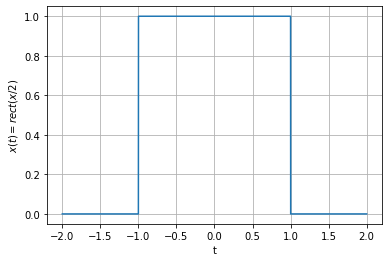
\includegraphics[width=\columnwidth]{solutions/ec/2008/32/figs/rect.png}
 \caption{Plot of x(t)}
 \label{ec/2008/32/plot}
\end{figure}
\begin{figure}[!h]
 \centering
 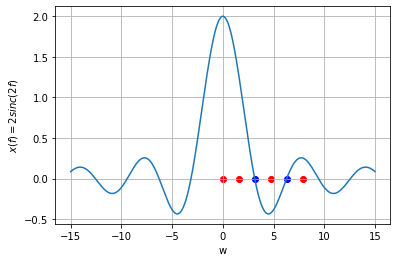
\includegraphics[width=\columnwidth]{solutions/ec/2008/32/figs/sinc.png}
 \caption{Plot of the fourier transform}
 \label{ec/2008/32/plot2}
\end{figure}

